\documentclass[aspectratio=169,10pt]{beamer}

\usepackage[T1]{fontenc}
\usepackage[utf8]{inputenc}
\usepackage{amsmath,amssymb,bm}
\usepackage{booktabs}
\usepackage{graphicx}
\usepackage{tikz}
\usepackage{xcolor}
\usepackage{helvet}
\usepackage{lmodern}
\usepackage{ragged2e}
\usefonttheme{professionalfonts}
\renewcommand{\familydefault}{\sfdefault}

\usetikzlibrary{arrows.meta,calc,decorations.pathreplacing,positioning}

\definecolor{Navy}{HTML}{163A5F}
\definecolor{PhysicsBlue}{HTML}{1F4E79}
\definecolor{MLOrange}{HTML}{B86118}
\definecolor{GateGreen}{HTML}{2F6F3E}
\definecolor{HarmRed}{HTML}{A23A35}
\definecolor{TextInk}{HTML}{202733}
\definecolor{MutedGray}{HTML}{666D78}
\definecolor{LineGray}{HTML}{C8CDD4}
\definecolor{SoftBlue}{HTML}{EEF4FA}
\definecolor{SoftOrange}{HTML}{F9EFE6}
\definecolor{SoftGreen}{HTML}{EAF4EE}
\definecolor{SoftRed}{HTML}{F8ECEA}
\definecolor{SoftGray}{HTML}{F4F5F7}

\setbeamercolor{background canvas}{bg=white}
\setbeamercolor{normal text}{fg=TextInk}
\setbeamercolor{frametitle}{fg=Navy,bg=white}
\setbeamercolor{title}{fg=Navy}
\setbeamertemplate{navigation symbols}{}
\setbeamersize{text margin left=0.70cm,text margin right=0.70cm}
\setbeamertemplate{footline}{%
  \hfill{\color{MutedGray}\scriptsize\insertframenumber}\hspace{0.45cm}\vspace{0.18cm}
}
\setbeamertemplate{frametitle}{%
  \vspace{0.18cm}
  {\Large\bfseries\insertframetitle}\par
  \vspace{0.07cm}
  {\color{LineGray}\rule{\textwidth}{0.6pt}}
  \vspace{-0.04cm}
}

\newcommand{\smallnote}[1]{\vspace{0.05cm}{\scriptsize\color{MutedGray}#1}}
\newcommand{\takeaway}[1]{%
  \vfill
  {\color{LineGray}\rule{\textwidth}{0.5pt}}\par
  \vspace{0.04cm}
  {\footnotesize\bfseries #1}
}
\newcommand{\plainbox}[4]{%
  \begin{tikzpicture}
    \node[
      draw=#1,
      fill=#2,
      line width=0.75pt,
      inner xsep=4pt,
      inner ysep=5pt,
      align=left
    ] {\parbox{#3}{\hyphenpenalty=10000\exhyphenpenalty=10000\emergencystretch=1em #4}};
  \end{tikzpicture}
}
\newcommand{\policycol}[4]{%
  \begin{tikzpicture}
    \node[
      draw=#1,
      fill=#2,
      line width=0.85pt,
      minimum width=0.93\linewidth,
      minimum height=3.72cm,
      inner xsep=7pt,
      inner ysep=8pt,
      align=left
    ] {\parbox{0.86\linewidth}{\hyphenpenalty=10000\exhyphenpenalty=10000\emergencystretch=1em\centering\normalsize\bfseries #3\par\vspace{0.16cm}\RaggedRight\small #4}};
  \end{tikzpicture}
}

\begin{document}

% Main slide 1
\begin{frame}[plain]
  \vspace{0.42cm}
  \begin{center}
    {\LARGE\bfseries When Not to Learn:}\\[2pt]
    {\LARGE\bfseries Evidence-Gated Residuals for LR-FHSS D2S IoT}\\[0.26cm]
    {\Large\bfseries\color{Navy} A real-data negative result on BLACK KITE TLE histories}\\[0.34cm]
    {\normalsize Anonymous Author 1 \quad Anonymous Author 2 \quad Anonymous Author 3}\\[0.06cm]
    {\small Affiliation omitted for double-blind review}\\
    {\small Email omitted}\\[0.32cm]
    {\scriptsize Advisor review / workshop draft}\\[0.42cm]
    {\Large\bfseries Residual ML must earn deployment; real evidence retains SGP4.}
  \end{center}
\end{frame}

% Main slide 2
\begin{frame}{Motivation and System Problem}
\begin{columns}[T,onlytextwidth]
    \column{0.58\textwidth}
    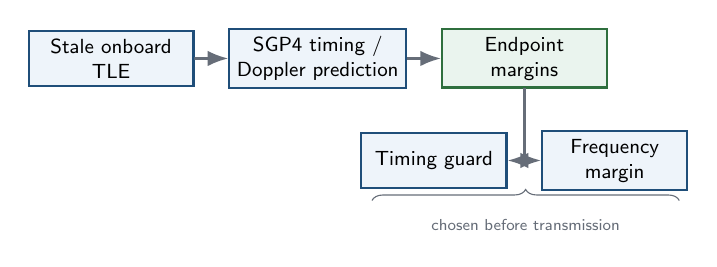
\begin{tikzpicture}[
      scale=0.82,
      transform shape,
      font=\small,
      >=Latex,
      stagebox/.style={draw=PhysicsBlue,fill=SoftBlue,line width=0.8pt,minimum width=2.55cm,minimum height=0.85cm,align=center},
      outbox/.style={draw=GateGreen,fill=SoftGreen,line width=0.8pt,minimum width=2.55cm,minimum height=0.85cm,align=center},
      arr/.style={->,line width=1.0pt,draw=MutedGray}
    ]
      \node[stagebox] (tle) at (0,2.0) {Stale onboard\\TLE};
      \node[stagebox] (sgp4) at (3.2,2.0) {SGP4 timing /\\Doppler prediction};
      \node[outbox] (margin) at (6.4,2.0) {Endpoint\\margins};
      \node[stagebox,minimum width=2.25cm] (time) at (5.0,0.42) {Timing guard};
      \node[stagebox,minimum width=2.25cm] (freq) at (7.8,0.42) {Frequency\\margin};
      \draw[arr] (tle) -- (sgp4);
      \draw[arr] (sgp4) -- (margin);
      \draw[arr] (margin.south) |- (time.east);
      \draw[arr] (margin.south) |- (freq.west);
      \draw[decorate,decoration={brace,amplitude=4pt},draw=MutedGray]
        (4.04,-0.20) -- node[below=5pt,align=center,text=MutedGray] {\scriptsize chosen before transmission} (8.80,-0.20);
    \end{tikzpicture}

    \vspace{0.32cm}
    {\large\bfseries Endpoint question}\\[2pt]
    {\normalsize Should a resource-constrained terminal deploy a learned inter-TLE residual correction over its available SGP4 baseline?}

    \column{0.38\textwidth}
    \plainbox{PhysicsBlue}{SoftBlue}{0.88\linewidth}{\normalsize
      The endpoint has orbital metadata, not a link outcome.
      It must size timing and frequency margins before the burst.}\\[0.20cm]
    \plainbox{MutedGray}{SoftGray}{0.88\linewidth}{\small
      Context: LR-FHSS direct-to-\linebreak satellite operation couples orbital prediction error to endpoint resource choices.}
  \end{columns}
  \takeaway{The control decision is pre-transmission: stale TLE to prediction to endpoint margins.}
  \smallnote{Selected context: Semtech AN1200.64; Ullah et al., OJ-COMS 2024.}
\end{frame}

% Main slide 3
\begin{frame}{Research Gap}
  \vspace{0.06cm}
\begin{columns}[T,onlytextwidth]
    \column{0.31\textwidth}
    {\bfseries LR-FHSS link / capacity}\\[-1pt]
    {\color{LineGray}\rule{\linewidth}{0.5pt}}\\[3pt]
    {\small Reliability, coverage, collision, and direct-to-satellite capacity studies.}\\[6pt]
    {\scriptsize\color{MutedGray}Semtech AN1200.64; Ullah WCL; LoRa D2S uplink policies}

    \column{0.31\textwidth}
    {\bfseries NTN synchronization}\\[-1pt]
    {\color{LineGray}\rule{\linewidth}{0.5pt}}\\[3pt]
    {\small Receiver-side synchronization and NTN mobility robustness.}\\[6pt]
    {\scriptsize\color{MutedGray}3GPP TR 38.821; Ullah OJ-COMS}

    \column{0.31\textwidth}
    {\bfseries Orbit / physics-ML correction}\\[-1pt]
    {\color{LineGray}\rule{\linewidth}{0.5pt}}\\[3pt]
    {\small SGP4, orbit prediction, differentiable propagation, and residual modeling.}\\[6pt]
    {\scriptsize\color{MutedGray}Hoots-Roehrich; Peng et al.; differentiable SGP4; ML orbit survey}
  \end{columns}
  \vspace{0.34cm}
  \plainbox{Navy}{white}{0.94\linewidth}{\normalsize
    \textbf{Gap.} Prior work predicts, receives, or schedules; it does not decide whether a resource-constrained endpoint should deploy learned inter-TLE correction over its available SGP4 baseline.}
  \takeaway{The missing object is a deployment rule, not another predictor leaderboard.}
\end{frame}

% Main slide 4
\begin{frame}{Hypothesis and Failure Risk}
\begin{columns}[T,onlytextwidth]
    \column{0.58\textwidth}
    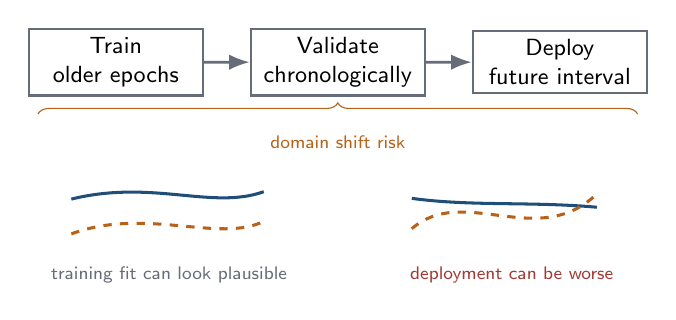
\begin{tikzpicture}[
      scale=0.94,
      transform shape,
      font=\small,
      >=Latex,
      phase/.style={draw=MutedGray,fill=white,line width=0.8pt,minimum width=2.35cm,minimum height=0.80cm,align=center},
      arr/.style={->,line width=1.0pt,draw=MutedGray}
    ]
      \node[phase] (train) at (0,2.2) {Train\\older epochs};
      \node[phase] (valid) at (3.0,2.2) {Validate\\chronologically};
      \node[phase] (deploy) at (6.0,2.2) {Deploy\\future interval};
      \draw[arr] (train) -- (valid);
      \draw[arr] (valid) -- (deploy);
      \draw[decorate,decoration={brace,amplitude=4pt},draw=MLOrange]
        (-1.05,1.50) -- node[below=5pt,text=MLOrange] {\scriptsize domain shift risk} (7.05,1.50);

      \draw[PhysicsBlue,line width=1.1pt] (-0.6,0.35) .. controls (0.5,0.62) and (1.3,0.20) .. (2.0,0.45);
      \draw[MLOrange,line width=1.1pt,dashed] (-0.6,-0.12) .. controls (0.4,0.25) and (1.4,-0.25) .. (2.0,0.05);
      \node[align=left,text=MutedGray] at (0.72,-0.68) {\scriptsize training fit can look plausible};

      \draw[PhysicsBlue,line width=1.1pt] (4.0,0.36) .. controls (4.8,0.25) and (5.6,0.32) .. (6.5,0.24);
      \draw[MLOrange,line width=1.1pt,dashed] (4.0,-0.05) .. controls (4.7,0.56) and (5.7,-0.35) .. (6.5,0.42);
      \node[align=left,text=HarmRed] at (5.35,-0.68) {\scriptsize deployment can be worse};
    \end{tikzpicture}

    \column{0.34\textwidth}
    {\bfseries Hypothesis}\\[3pt]
    {\normalsize Residuals may be learnable.}\\[0.30cm]
    {\bfseries Failure risk}\\[3pt]
    {\normalsize Chronological shift can make always-on ML worse than SGP4.}\\[0.30cm]
    \plainbox{HarmRed}{SoftRed}{0.92\linewidth}{\small
      A plausible learner remains unsafe until it wins on held-out \mbox{chronological} evidence.}
  \end{columns}
  \takeaway{Learning enters as an untrusted candidate.}
\end{frame}

% Main slide 5
\begin{frame}{Method: Evidence Gate}
  \vspace{0.10cm}
  \begin{center}
    {\LARGE$\displaystyle
      G=\mathbf{1}\!\left[
      \mathrm{MAE}_{\mathrm{ml}}(V)
      < \gamma\,\mathrm{MAE}_{\mathrm{phys}}(V)
      \right]$}
  \end{center}
  \vspace{0.18cm}
\begin{columns}[T,onlytextwidth]
    \column{0.54\textwidth}
    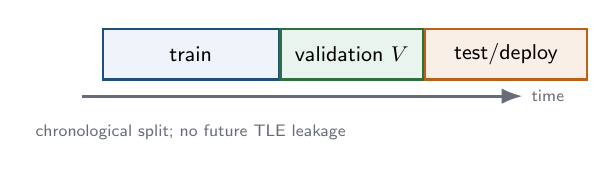
\begin{tikzpicture}[
      scale=0.86,
      transform shape,
      font=\small,
      train/.style={draw=PhysicsBlue,fill=SoftBlue,line width=0.8pt,minimum height=0.75cm,align=center},
      valid/.style={draw=GateGreen,fill=SoftGreen,line width=0.8pt,minimum height=0.75cm,align=center},
      test/.style={draw=MLOrange,fill=SoftOrange,line width=0.8pt,minimum height=0.75cm,align=center},
      >=Latex
    ]
      \node[train,minimum width=2.6cm] (tr) at (0,0) {train};
      \node[valid,minimum width=2.1cm,right=0pt of tr] (va) {validation $V$};
      \node[test,minimum width=2.4cm,right=0pt of va] (te) {test/deploy};
      \draw[->,line width=1.0pt,draw=MutedGray] (-1.6,-0.62) -- (4.9,-0.62)
        node[right,text=MutedGray] {\scriptsize time};
      \node[align=center,text=MutedGray] at (0,-1.15) {\scriptsize chronological split; no future TLE leakage};
    \end{tikzpicture}

    \vspace{0.30cm}
    {\scriptsize\color{MutedGray} Training fits the candidates. $G$ is fixed on validation; the test segment only reports consequences. MAE is the gate loss; RMSE is a diagnostic, not part of the rule.}

    \column{0.42\textwidth}
    {\bfseries What $\gamma$ does}\\[3pt]
    {\small Smaller $\gamma$ demands a clearer held-out gain. It reduces false-open risk at the cost of missed-open opportunities.}\\[0.10cm]
    \smallnote{$\gamma = 0.95$ in all experiments.}\\[0.20cm]
    \plainbox{GateGreen}{SoftGreen}{0.90\linewidth}{\small
      Audit rule, not a new predictor. The deployable baseline remains SGP4 unless the learner earns the branch.}
  \end{columns}
  \takeaway{The rule decides whether learned correction may deploy over the available baseline.}
\end{frame}

% Main slide 6
\begin{frame}{Experimental Protocol}
\begin{columns}[T,onlytextwidth]
    \column{0.50\textwidth}
    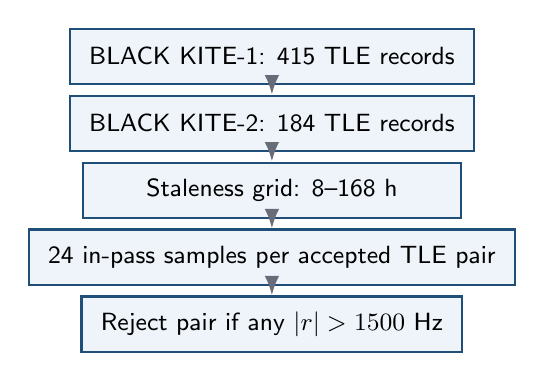
\begin{tikzpicture}[
      font=\small,
      >=Latex,
      item/.style={draw=PhysicsBlue,fill=SoftBlue,line width=0.8pt,minimum width=4.8cm,minimum height=0.70cm,align=left,inner xsep=7pt},
      arr/.style={->,line width=0.9pt,draw=MutedGray}
    ]
      \node[item] (a) at (0,2.8) {BLACK KITE-1: 415 TLE records};
      \node[item] (b) at (0,1.95) {BLACK KITE-2: 184 TLE records};
      \node[item] (c) at (0,1.10) {Staleness grid: 8--168 h};
      \node[item] (d) at (0,0.25) {24 in-pass samples per accepted TLE pair};
      \node[item] (e) at (0,-0.60) {Reject pair if any $|r|>1500$ Hz};
      \draw[arr] (a) -- (b);
      \draw[arr] (b) -- (c);
      \draw[arr] (c) -- (d);
      \draw[arr] (d) -- (e);
    \end{tikzpicture}

    \vspace{0.34cm}
    {\scriptsize\color{MutedGray} The real claim is conditional on accepted non-outlier pairs; $|r|>1500$ Hz pairs are excluded and left for a maneuver/outlier extension.}

    \column{0.46\textwidth}
    {\bfseries Chronological split}\\[0.08cm]
    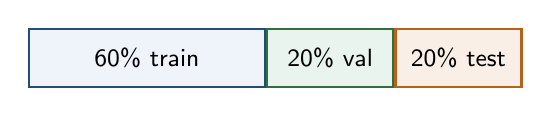
\begin{tikzpicture}[
      font=\small,
      tr/.style={draw=PhysicsBlue,fill=SoftBlue,line width=0.8pt,minimum height=0.74cm,align=center},
      va/.style={draw=GateGreen,fill=SoftGreen,line width=0.8pt,minimum height=0.74cm,align=center},
      te/.style={draw=MLOrange,fill=SoftOrange,line width=0.8pt,minimum height=0.74cm,align=center}
    ]
      \node[tr,minimum width=3.0cm] (tr) at (0,0) {60\% train};
      \node[va,minimum width=1.6cm,right=0pt of tr] (va) {20\% val};
      \node[te,minimum width=1.6cm,right=0pt of va] (te) {20\% test};
    \end{tikzpicture}

    \vspace{0.30cm}
    {\bfseries Reference boundary}\\[3pt]
    {\small \texttt{reference\_is\_measured\_truth=false}. All real results are model-derived inter-TLE residuals.}\\[0.28cm]
    {\bfseries Candidate models}\\[3pt]
    {\small Ridge, random forest, gradient boosting, and small MLP selected on validation.}
  \end{columns}
  \takeaway{The real-data protocol tests deployable chronological utility, not measured Doppler truth.}
\end{frame}

% Main slide 7
\begin{frame}{Main Real Result}
  \vspace{-0.25cm}
  \begin{center}
    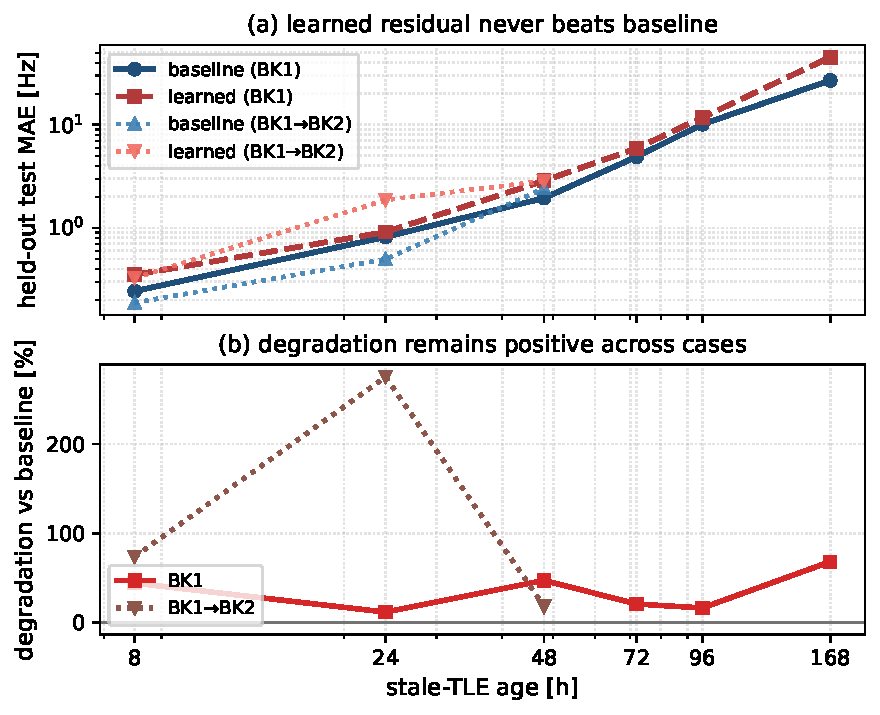
\includegraphics[width=0.99\linewidth,height=0.66\textheight,keepaspectratio]{figures/fig_bk_residual_talk.pdf}
  \end{center}
  \vspace{-0.46cm}
  {\footnotesize\bfseries All reported BLACK KITE point estimates close the gate; deploy SGP4 / never-learn.}\\[1pt]
  {\scriptsize\color{MutedGray} Reported point estimates are worse in every row; BK1 degradation 11.6\%--68.1\%. Cross-satellite rows (up to 275.1\%) are a limited transfer check; per-split counts were not preserved. Point estimates under the leakage-free protocol; not pair-clustered inference.}
\end{frame}

% Main slide 8
\begin{frame}{Why a Closed Gate Matters}
  \vspace{0.04cm}
\begin{columns}[T,onlytextwidth]
    \column{0.31\textwidth}
    \policycol{HarmRed}{SoftRed}{Always learn}{Deploys the learned branch by default.\par\vspace{0.20cm}On BLACK KITE, this increases residual error.}

    \column{0.31\textwidth}
    \policycol{PhysicsBlue}{SoftBlue}{Never learn}{Retains the SGP4 stale-TLE baseline.\par\vspace{0.20cm}On BLACK KITE, this is the selected safe output.}

    \column{0.31\textwidth}
    \policycol{GateGreen}{SoftGreen}{Evidence Gate}{Tests the learned branch on chronological validation.\par\vspace{0.20cm}On BLACK KITE, it chooses the same output as never-learn.}
  \end{columns}
  \vspace{0.22cm}
  \begin{center}
    \plainbox{Navy}{white}{0.93\linewidth}{\small
      At BK1 168 h, 26.9 $\to$ 45.3 Hz is still $\ll F_{\mathrm{tol}} = 500$ Hz: this is a refusal/audit result, not an energy-win claim.}
  \end{center}
  \takeaway{Gate value here is auditability: it blocks unsupported always-on ML, not guaranteed improvement.}
\end{frame}

% Main slide 9
\begin{frame}{Controlled Synthetic Mechanism Check}
\begin{columns}[T,onlytextwidth]
    \column{0.54\textwidth}
    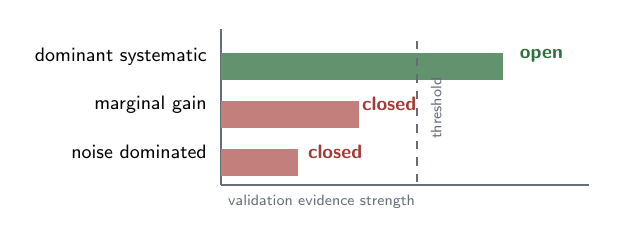
\begin{tikzpicture}[
      scale=0.78,
      transform shape,
      font=\small,
      y=0.82cm,
      >=Latex,
      bar/.style={minimum height=0.44cm,anchor=west},
      axis/.style={draw=MutedGray,line width=0.75pt}
    ]
      \draw[axis] (0,0) -- (6.0,0);
      \draw[axis] (0,0) -- (0,3.1);
      \node[anchor=east] at (-0.10,2.55) {dominant systematic};
      \node[anchor=east] at (-0.10,1.60) {marginal gain};
      \node[anchor=east] at (-0.10,0.65) {noise dominated};
      \node[bar,fill=GateGreen!75,minimum width=4.6cm] at (0,2.34) {};
      \node[bar,fill=HarmRed!65,minimum width=2.25cm] at (0,1.39) {};
      \node[bar,fill=HarmRed!65,minimum width=1.25cm] at (0,0.44) {};
      \draw[dashed,draw=MutedGray,line width=0.9pt] (3.20,0.05) -- (3.20,3.0);
      \node[rotate=90,anchor=south,text=MutedGray] at (3.72,1.52) {\scriptsize threshold};
      \node[anchor=west,text=GateGreen] at (4.75,2.56) {\bfseries open};
      \node[anchor=west,text=HarmRed] at (2.18,1.61) {\bfseries closed};
      \node[anchor=west,text=HarmRed] at (1.30,0.66) {\bfseries closed};
      \node[anchor=west,text=MutedGray] at (0,-0.34) {\scriptsize validation evidence strength};
    \end{tikzpicture}

    \column{0.38\textwidth}
    \plainbox{Navy}{white}{0.92\linewidth}{\small
      \textbf{Controlled software-only check.}\\[3pt]
      Synthetic cases open only when a dominant systematic residual is present.}\\[0.25cm]
    {\small
      Noise dominated: closed.\\[3pt]
      Marginal gain below $\gamma$: closed.\\[3pt]
      Dominant systematic residual: open.}
  \end{columns}
  \takeaway{Synthetic evidence checks mechanism only.}
\end{frame}

% Main slide 10
\begin{frame}{Endpoint Implications}
\begin{columns}[T,onlytextwidth]
    \column{0.62\textwidth}
    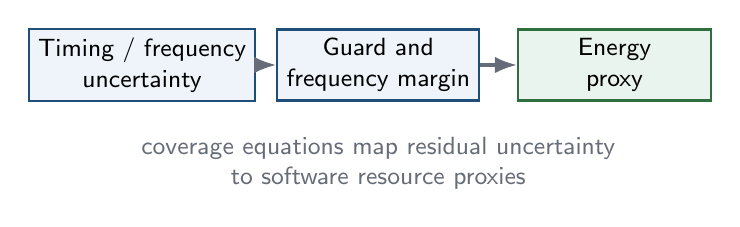
\begin{tikzpicture}[
      font=\small,
      >=Latex,
      proxybox/.style={draw=PhysicsBlue,fill=SoftBlue,line width=0.8pt,minimum width=2.45cm,minimum height=0.82cm,align=center},
      proxygreen/.style={draw=GateGreen,fill=SoftGreen,line width=0.8pt,minimum width=2.45cm,minimum height=0.82cm,align=center},
      arr/.style={->,line width=1.1pt,draw=MutedGray}
    ]
      \node[proxybox] (u) at (0,1.5) {Timing / frequency\\uncertainty};
      \node[proxybox] (g) at (3.0,1.5) {Guard and\\frequency margin};
      \node[proxygreen] (e) at (6.0,1.5) {Energy\\proxy};
      \draw[arr] (u) -- (g);
      \draw[arr] (g) -- (e);
      \node[align=center,text=MutedGray] at (3.0,0.25) {\small coverage equations map residual uncertainty\\to software resource proxies};
    \end{tikzpicture}

    \vspace{0.28cm}
    \plainbox{HarmRed}{SoftRed}{0.90\linewidth}{\small
      Software-only control proxy; not a packet result.\\[2pt]
      Proxy scale is illustrative: it is not the BLACK KITE residual scale and not a link result.}

    \column{0.34\textwidth}
    {\bfseries Design implication}\\[3pt]
    {\small A learner that does not win the gate should not consume extra guard, frequency margin, or energy budget.}\\[0.30cm]
    {\bfseries Audit implication}\\[3pt]
    {\small The deployed policy must record why the learned branch was allowed or blocked.}
  \end{columns}
  \takeaway{The proxy connects residual evidence to endpoint budget pressure without field-result evidence.}
\end{frame}

% Main slide 11
\begin{frame}{Limitations and Next Campaign}
\begin{columns}[T,onlytextwidth]
    \column{0.47\textwidth}
    {\bfseries Current limitations}\\[-1pt]
    {\color{LineGray}\rule{\linewidth}{0.5pt}}\\[5pt]
    {\normalsize
    \begin{itemize}
      \item Two BLACK KITE satellites
      \item Model-derived reference only; no measured Doppler truth
      \item Oscillator and channel effects may dominate practical endpoints
      \item MAE gate is not tail-aware
    \end{itemize}}

    \column{0.47\textwidth}
    {\bfseries Next software campaign}\\[-1pt]
    {\color{LineGray}\rule{\linewidth}{0.5pt}}\\[5pt]
    {\normalsize
    \begin{itemize}
      \item Multi-satellite TLE stress matrix
      \item Residual autocorrelation and learnability analysis
      \item Stronger baselines
      \item Tail-aware or cost-aware gate
    \end{itemize}}
  \end{columns}
  \takeaway{Broader deployment value requires broader chronological evidence and a loss beyond MAE.}
\end{frame}

% Main slide 12
\begin{frame}{Contributions and Takeaway}
  \vspace{0.05cm}
  \begin{enumerate}
    \setlength{\itemsep}{0.34cm}
    \item \textbf{Real-data negative finding.} On BLACK KITE TLE history, the reported inter-TLE point estimates are worse than SGP4 in every row.
    \item \textbf{Evidence-gated deploy/refuse audit rule.} $G$ is decided on chronological validation; on real BLACK KITE data the gate closes and deployment equals SGP4 / never-learn.
    \item \textbf{Secondary: illustrative endpoint-budget proxy.} Timing, frequency, and energy figures are software-only coverage proxies, not packet or field results.
  \end{enumerate}
  \vspace{0.35cm}
  \begin{center}
    {\Large\bfseries Do not trust residual ML by default.}\\[4pt]
    {\Large\bfseries Let chronological evidence decide deployment.}
  \end{center}
\end{frame}

\appendix

% Backup slide 1
\begin{frame}{Backup: Endpoint Proxy Ablation}
  \begin{center}
    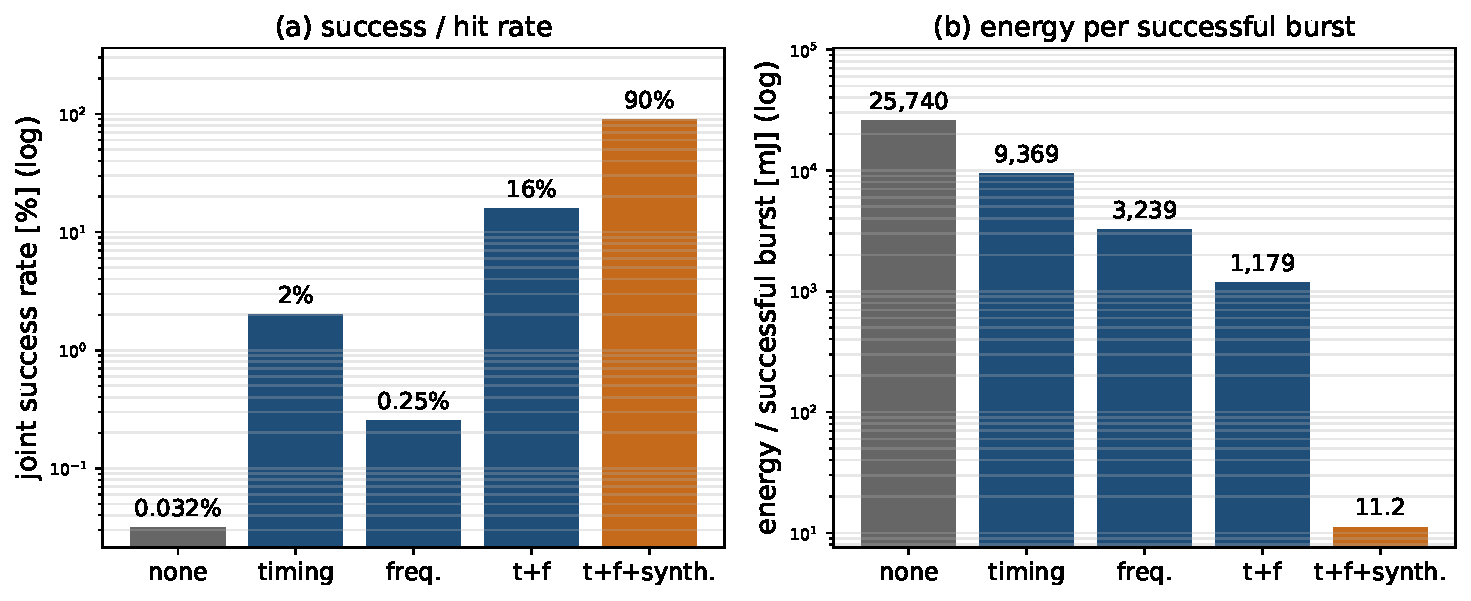
\includegraphics[width=0.80\linewidth,height=0.50\textheight,keepaspectratio]{slide_figures/fig_control_ablation_talk.pdf}
  \end{center}
  \plainbox{Navy}{white}{0.88\linewidth}{\scriptsize
    Detailed software-only proxy ablation. The orange right-most bar (\texttt{t+f+synth.}) is the synthetic gate-open branch, not a BLACK KITE improvement.}
\end{frame}

% Backup slide 2
\begin{frame}{Backup: Counts and Gate Sensitivity}
\begin{columns}[T,onlytextwidth]
    \column{0.47\textwidth}
    {\bfseries Experimental counts}\\[-1pt]
    {\color{LineGray}\rule{\linewidth}{0.5pt}}\\[4pt]
    {\small
    \begin{tabular}{@{}ll@{}}
      \toprule
      BLACK KITE-1 & 415 TLE records \\
      BLACK KITE-2 & 184 TLE records \\
      Samples & 24 per accepted pair \\
      Split & chronological 60/20/20 \\
      Staleness & 8--168 h \\
      Reject rule & any $|r|>1500$ Hz \\
      \bottomrule
    \end{tabular}}

    \column{0.47\textwidth}
    {\bfseries Gate interpretation}\\[-1pt]
    {\color{LineGray}\rule{\linewidth}{0.5pt}}\\[4pt]
    {\small
    \begin{itemize}
      \item Lower $\gamma$ demands larger validation gain.
      \item False-open risk: deploying a harmful learned branch.
      \item Missed-open risk: retaining SGP4 despite real systematic gain.
      \item Real BLACK KITE rows close under the tested settings.
    \end{itemize}}
  \end{columns}
  \takeaway{The sensitivity question is policy conservatism, not predictor novelty.}
\end{frame}

% Backup slide 3
\begin{frame}{Backup: Software Extension Diagnostics}
  \vspace{0.06cm}
\begin{columns}[T,onlytextwidth]
    \column{0.49\textwidth}
    {\bfseries What the extension confirms}\\[-1pt]
    {\color{LineGray}\rule{\linewidth}{0.5pt}}\\[5pt]
    {\small
    \begin{itemize}
      \item Lightweight bias and baseline variants still do not beat SGP4 on BLACK KITE.
      \item The real MAE gate remains closed in every reported row.
    \end{itemize}}
    \vspace{0.16cm}
    \plainbox{PhysicsBlue}{SoftBlue}{0.90\linewidth}{\scriptsize
      Median bias, ridge, random forest, gradient boosting, and small MLP; summary-level audit of committed artifacts, not fresh retraining.}

    \column{0.49\textwidth}
    {\bfseries What it does not establish}\\[-1pt]
    {\color{LineGray}\rule{\linewidth}{0.5pt}}\\[5pt]
    {\small
    \begin{itemize}
      \item A tail-aware real gate needs per-sample prediction export; not claimed here.
      \item The multi-satellite pipeline is prepared as future work; no new generalization claim.
    \end{itemize}}
    \vspace{0.16cm}
    \plainbox{MutedGray}{SoftGray}{0.90\linewidth}{\scriptsize
      All rows are software-only, model-derived inter-TLE results.}
  \end{columns}
  \takeaway{The extension reinforces the same safe decision; it does not widen the claim.}
\end{frame}

% Backup slide 4
\begin{frame}{Backup: What This Work Does Not Claim}
  \vspace{0.16cm}
  {\normalsize
  \begin{itemize}
    \setlength{\itemsep}{0.20cm}
    \item No measured Doppler truth; the reference is a later TLE propagated by SGP4.
    \item No packet-level, decoding, error-rate, or receiver-acknowledgement outcome.
    \item No over-the-air transmission and no on-orbit result.
    \item The synthetic gate-open case is a mechanism check, not a real-data improvement.
    \item Endpoint proxy curves are software-only; they are not a link-layer result.
  \end{itemize}}
  \vspace{0.22cm}
  \begin{center}
    \plainbox{HarmRed}{SoftRed}{0.90\linewidth}{\small
      The claim is a deployment decision on model-derived inter-TLE residuals: on BLACK KITE, keep SGP4 / never-learn.}
  \end{center}
\end{frame}

\end{document}
